% !TEX program = xelatex
\documentclass[a4paper,14pt,oneside,openany]{memoir}

%%% Задаем поля, отступы и межстрочный интервал %%%

\usepackage[left=30mm, right=15mm, top=20mm, bottom=20mm]{geometry}
\pagestyle{plain}
\parindent=1.25cm
\usepackage{indentfirst}

%%% Задаем языковые параметры и шрифт %%%

\usepackage[english,russian]{babel}
\babelfont[russian]{rm}{Times New Roman}
\babelfont[russian]{tt}{Courier New}

%%% Задаем стиль заголовков и подзаголовков в тексте %%%

\setsecnumdepth{subsection}
\renewcommand*{\chapterheadstart}{}
\renewcommand*{\printchaptername}{}
\renewcommand*{\chapnumfont}{\normalfont\bfseries}
\renewcommand*{\afterchapternum}{\hspace{1em}}
\renewcommand*{\printchaptertitle}[1]{\normalfont\bfseries\centering\MakeUppercase{#1}}
\setbeforesecskip{20pt}
\setaftersecskip{20pt}
\setsecheadstyle{\raggedright\normalfont\bfseries}
\setbeforesubsecskip{20pt}
\setaftersubsecskip{20pt}
\setsubsecheadstyle{\raggedright\normalfont\bfseries}

%%% Исправление нумерации секций %%%

\renewcommand{\thesection}{\arabic{section}}
\renewcommand{\thesubsection}{\arabic{subsection}}

%%% Сквозная нумерация рисунков и таблиц %%%

\counterwithout{figure}{chapter}
\counterwithout{table}{chapter}

%%% Выравнивание и переносы %%%

\tolerance 1414
\hbadness 1414
\emergencystretch 1.5em
\clubpenalty=10000
\widowpenalty=10000

%%% Задаем параметры оформления рисунков и таблиц %%%

\usepackage{graphicx}
\usepackage{caption}
\usepackage{subcaption}
\usepackage{float}
\graphicspath{{photo/}}
\captionsetup[figure]{font=small, width=\textwidth, name=Рисунок, justification=centering}
\captiondelim{ --- }
\usepackage[section]{placeins}

%%% Задаем параметры ссылок и гиперссылок %%% 

\usepackage{hyperref}
\hypersetup{
    colorlinks=true,
    linkcolor=red,
    citecolor=red
}

%%% Настраиваем отображение списков %%%

\usepackage{enumitem}
\renewcommand*{\labelitemi}{\normalfont{--}}
\setlist{noitemsep, leftmargin=*}

%%% Для verbatim %%%
\usepackage{verbatim}

\begin{document}

% Титульный лист (без номера страницы)
\thispagestyle{empty}

\begin{center}
    МИНИСТЕРСТВО ЦИФРОВОГО РАЗВИТИЯ, СВЯЗИ И МАССОВЫХ \\ КОММУНИКАЦИЙ \\ РОССИЙСКОЙ ФЕДЕРАЦИИ

    \vspace{20pt}

    Федеральное государственное бюджетное образовательное учреждение \\ высшего образования \\
    "Сибирский государственный университет телекоммуникаций и \\ информатики"

    \vspace{20pt}

    Кафедра телекоммуникационных систем и вычислительных средств \\ (ТС и ВС)
\end{center}

\vfill

\begin{center}
    Практическая работа №7 \\
    по дисциплине \\
    \textit{"Web-технологии"}

    \vspace{20pt}

    по теме: \\
    \uppercase{Электронная почта (iRedMail)}
\end{center}

\vfill

\noindent Студент: \\
\textit{Группа ИКС-532 \hfill Шиф Д.А.}

\vspace{20pt}

\noindent Преподаватель: \\
\textit{старший преподаватель \hfill А.В. Андреев}

\vfill

\begin{center}
    Новосибирск 2026 г.
\end{center}

\newpage
\setcounter{page}{2}
\OnehalfSpacing*

\subsection*{Цель работы}

\begin{itemize}
    \item Настроить почтовый сервер iRedMail на отдельной виртуальной машине
    \item Настроить DNS-записи (A, MX, SPF) для домена SHIF.GROUP.internal
    \item Создать тестовых пользователей и проверить работу почты
\end{itemize}

\section{Введение}

В данной практической работе настраивается почтовый сервер iRedMail на отдельной виртуальной машине. iRedMail позволяет организовать полнофункциональный почтовый сервер с веб-интерфейсом администрирования и веб-почтой.

Параметры варианта:
\begin{itemize}
    \item Номер варианта: 20
    \item Подсеть: 192.168.20.0/24
    \item Домен: SHIF.GROUP.internal
    \item IP-адрес почтового сервера: 192.168.20.5
    \item IP-адрес шлюза: 192.168.20.1
\end{itemize}

\section{Ход работы}

\subsection{Создание и настройка виртуальной машины Mail}

Была создана виртуальная машина mail со статическим IP-адресом 192.168.20.5.

\begin{figure}[H]
    \centering
    
\includegraphics[width=0.7\textwidth]{/Users/artemlesin/lab8.c/Laba9/web-technology/me/lab7_1.jpg}
    \caption{Настройка сетевого интерфейса почтового сервера}
\end{figure}

\subsection{Добавление DNS-записей}

На шлюзе в конфигурацию DNS добавлены записи для почтового сервера:

\begin{verbatim}
mail IN A 192.168.20.5
@ IN MX 10 mail.SHIF.GROUP.internal.
@ IN TXT "v=spf1 a mx ip4:192.168.20.5 -all"
\end{verbatim}

\begin{figure}[H]
    \centering
    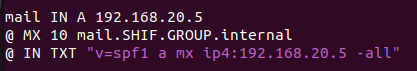
\includegraphics[width=0.7\textwidth]{lab7_2.png}
    \caption{DNS-записи для почтового сервера}
\end{figure}

\subsection{Установка iRedMail}

Установка выполнена с параметрами: Nginx, OpenLDAP, домен SHIF.GROUP.internal.

\begin{figure}[H]
    \centering
    
\includegraphics[width=0.7\textwidth]{lab7_3.png}
    \caption{Веб-интерфейс Roundcube после установки}
\end{figure}

\section{Результат работы}

Почтовый сервер доступен по адресу \href{https://mail.SHIF.GROUP.internal}{https://mail.SHIF.GROUP.internal}. Созданы тестовые пользователи, проверена отправка и получение писем.

\section*{Заключение}
\addcontentsline{toc}{section}{Заключение}

В ходе выполнения практической работы был развернут почтовый сервер iRedMail. Были выполнены следующие задачи:

\begin{enumerate}
    \item Создана виртуальная машина со статическим IP-адресом 192.168.20.5
    \item Настроены DNS-записи: A-запись, MX-запись, SPF-запись
    \item Установлен и настроен iRedMail с параметрами Nginx, OpenLDAP
    \item Созданы тестовые пользователи
    \item Проверена работоспособность почты через веб-интерфейс Roundcube
\end{enumerate}

Почта функционирует корректно. Задачи выполнены в полном объеме.

\end{document}